%!TEX root = ../dokumentation.tex

\chapter{Versuchsumgebung}
\label{section:versuchsumgebung}
Im folgenden Kapitel wird die Versuchsumgebung erläutert. Um einen Überblick über die Versuchsumgebung zu bekommen, wird zu Beginn der Aufbau der Umgebungen beschrieben. Danach werden die einzelnen Szenen vorgestellt, welche für die Versuchsdurchführung erstellt wurden. In dem Kapitel werden zudem die verschiedenen Steuerungsmöglichkeiten für die Versuche vorgestellt. Als Letztes wird die Implementierung erläutert. 

\section{Aufbau}
Um die Verwendung von Eye-Tracking zur Steuerung von Bedienelementen in \ac{VR} untersuchen zu können, finden die Versuche in einem leeren, neutralen Raum statt. Ein genereller Vorteil von Versuchen in \ac{VR} ist, dass die Versuche in einer digitalen Umgebung stattfinden. Dadurch wird die komplette Kontrolle über die Umgebung behalten und die Versuche sind stets wiederholbar. Der Versuch im leeren neutralen Raum hat den Vorteil, dass der Benutzer von der kompletten realen Welt abgeschirmt ist. Ein Nebeneffekt dabei ist, dass der Benutzer sich besser auf den Versuch fokussieren kann, da dieser nicht durch eventuell neu gewonnene Eindrücke aus der \ac{VR}-Welt abgelenkt wird. Um Ablenkungen bezüglich Farbwechsel an den Wänden, dem Boden oder der Decke zu vermeiden, erhalten diese Elemente die selbe Hintergrundfarbe. Zudem wird der Raum gleichmäßig beleuchtet. Für eine bessere Vergleichbarkeit der Versuchsergebnisse muss der Benutzer bei jedem Versuch auf der gleichen Position im Raum stehen. Diese Position wird auf dem Boden durch ein rotes Quadrat markiert (siehe \autoref{fig:game-plan}). Da der Benutzer die Möglichkeit hat, sich innerhalb einer vom \ac{VR}-Headset berechneten Spielfläche zu bewegen, muss sich der Benutzer vor dem Beginn des Versuches auf dem roten Quadrat positionieren. Dieses Quadrat befindet sich mittig zentriert circa eine halbe \acl{u} vor einer Wand. Das Quadrat hat eine Seitenlänge von einer halben \acl{u}.

Zur Untersuchung der Eignung von Eye-Tracking bei der Steuerung von Bedienelementen befindet sich auf der gegenüberliegenden Wand die Versuchsfläche (siehe \autoref{fig:game-view}). Der Versuch ist wie ein Spiel aufgebaut. Der Benutzer muss fünf zufällige Zahlen von 1 bis 16 nacheinander auswählen. Auf der Spielfläche befinden sich 16 Bedienelemente, die mit Zahlen von 1 bis 16 beschriftet sind. Oberhalb der Bedienelemente befindet sich ein Textfeld, welches dem Benutzer die auszuwählende Zahl mitteilt. Zudem teilt das Textfeld das Ende des Spieles mit. Um das Spiel zu starten, muss der Benutzer den GO-Knopf betätigen. Beim Betätigen eines Bedienelementes wird die Hintergrundfarbe des Elements verändert. Dies wird in Abhängigkeit der gesuchten Zahl und des ausgewählten Elements festgelegt. Wenn die gesuchte Zahl und die Beschriftung des ausgewählten Bedienelements übereinstimmen, wird das Element grün gefärbt, ansonsten rot. \\
Für die Untersuchung von Fitts's Law in \ac{VR} sind die Bedienelemente im Durchmesser verstellbar. Für die Versuche stehen drei verschiedene Skalierungen zur Verfügung. Der größte Durchmesser ist 0,4\ac{u} groß und der Skalierungsfaktor ist eins. Der mittlere Durchmesser wird mit dreiviertel des größten Durchmesser skaliert. Der kleinste Durchmesser ist nur noch halb so groß wie der Größte.

\begin{figure}[!htbp]
	\centering
	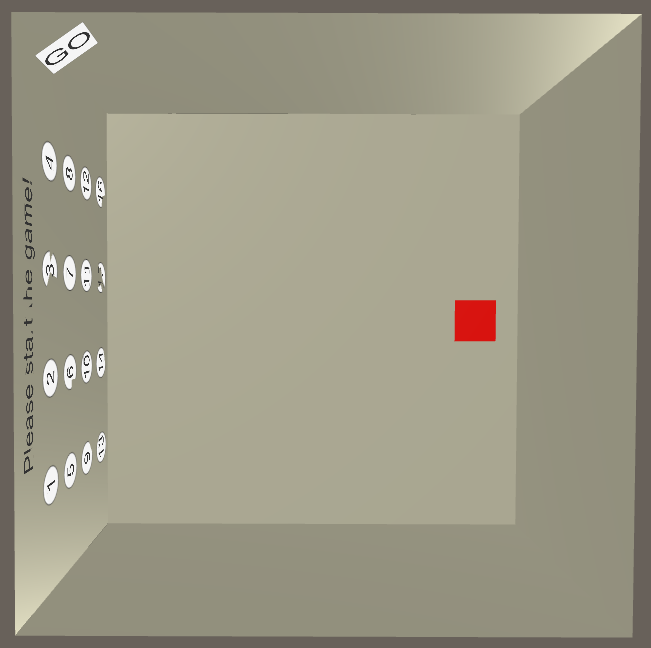
\includegraphics[width=0.65\linewidth]{game-plan}
	\caption[Draufsicht auf den Raum]{Draufsicht auf den Raum}
	\label{fig:game-plan}
\end{figure}

\begin{figure}[!htbp]
\centering
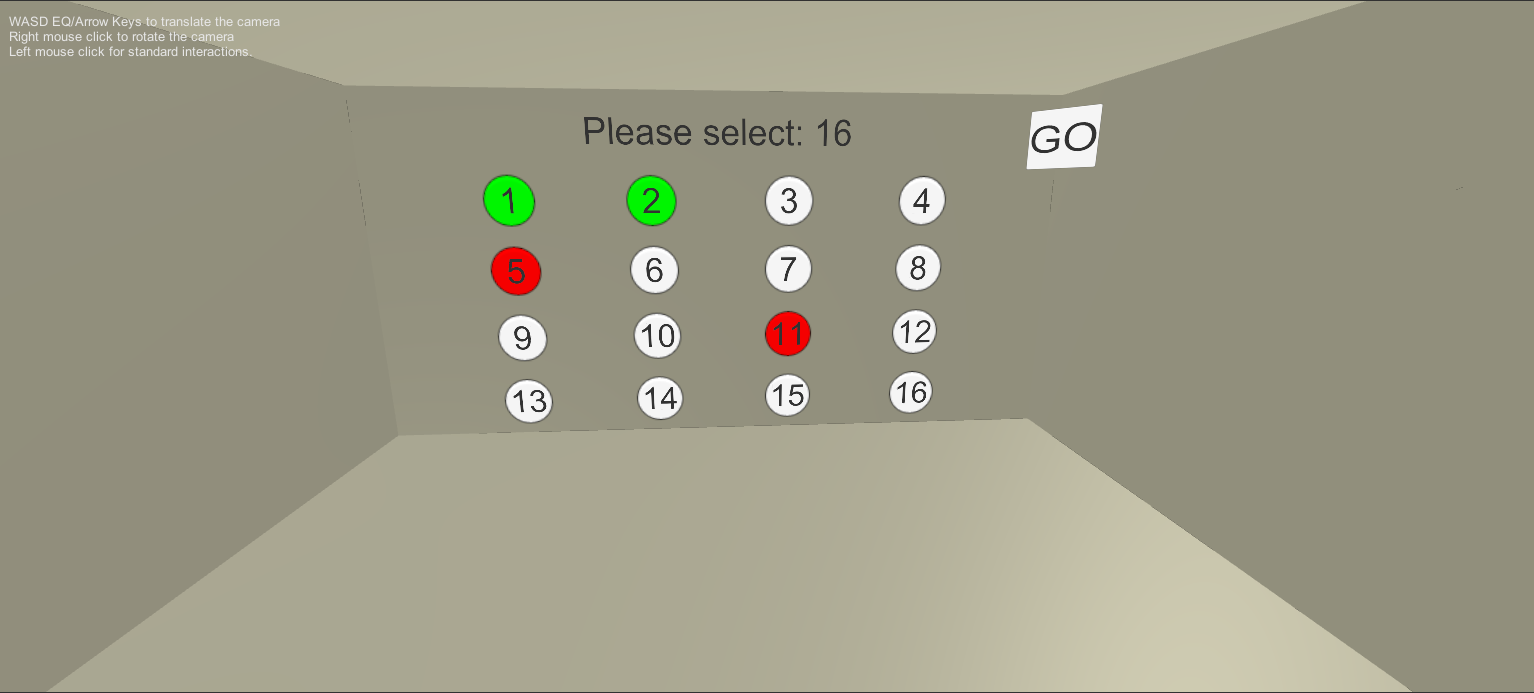
\includegraphics[width=1\linewidth]{game-view}
\caption[Benutzersicht auf den Versuch]{Benutzersicht auf den Versuch}
\label{fig:game-view}
\end{figure}

\section{Szenen}
Für die Versuche existieren vier verschiedene Szenen, in denen die Eignung von Eye-Tracking als Steuerung in \ac{VR} untersucht wird. Jede Szene basiert auf dem zuvor beschriebenen Aufbau. Jeder der Räume ist 2,5\ac{u} hoch und 5\ac{u} breit. Die Idee an den ersten drei Szenen ist, zu untersuchen, welchen Einfluss die Entfernung der Bedienelemente auf die Zuverlässigkeit des Eye-Trackings hat. Zudem wird in diesen drei Szenen Fitts' Gesetz in \ac{VR} mit Eye-Tracking untersucht. Die Namen der Szenen orientieren sich daher an Fitts's Law. In der ersten Szene \glqq FittsLaw\grqq{} (siehe \autoref{fig:game-view}) steht der Benutzer in einer Entfernung von 4,5\ac{u} zur Spielfläche. In der zweiten Szene \glqq FittsLawFar\grqq{} (siehe \autoref{fig:FittsLawFar}) und der dritten Szene \glqq FittsLawFurther\grqq{} (siehe \autoref{fig:FittsLawFurther}) vergrößert sich die Entfernung jeweils um 2,5\ac{u} zur vorherigen Szene. In der dritten Szene ist der Benutzer daher 9,5\ac{u} von der Spielfläche entfernt. 

\begin{figure}[!htbp]
	\centering
	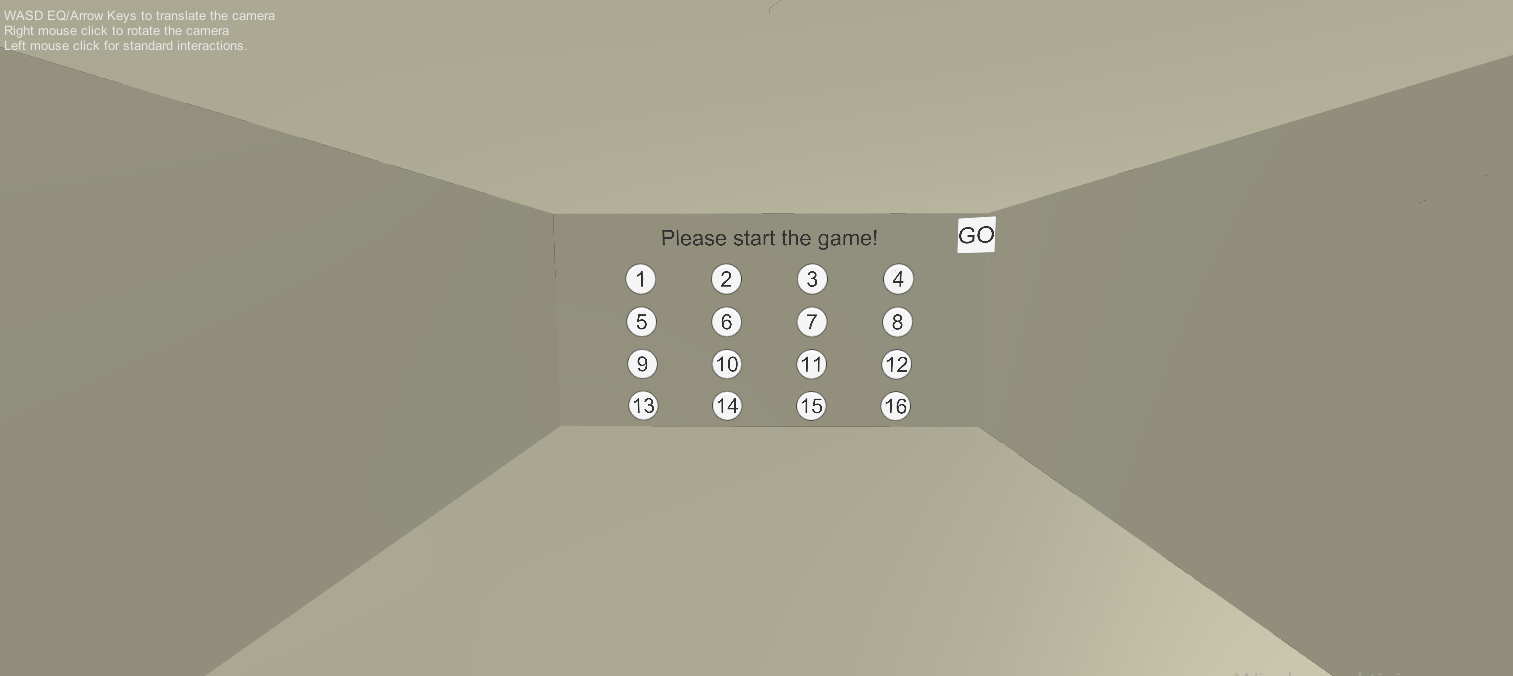
\includegraphics[width=1\linewidth]{FittsLawFar}
	\caption[Szene FittsLawFar]{Szene FittsLawFar}
	\label{fig:FittsLawFar}
\end{figure}

\begin{figure}[!htbp]
	\centering
	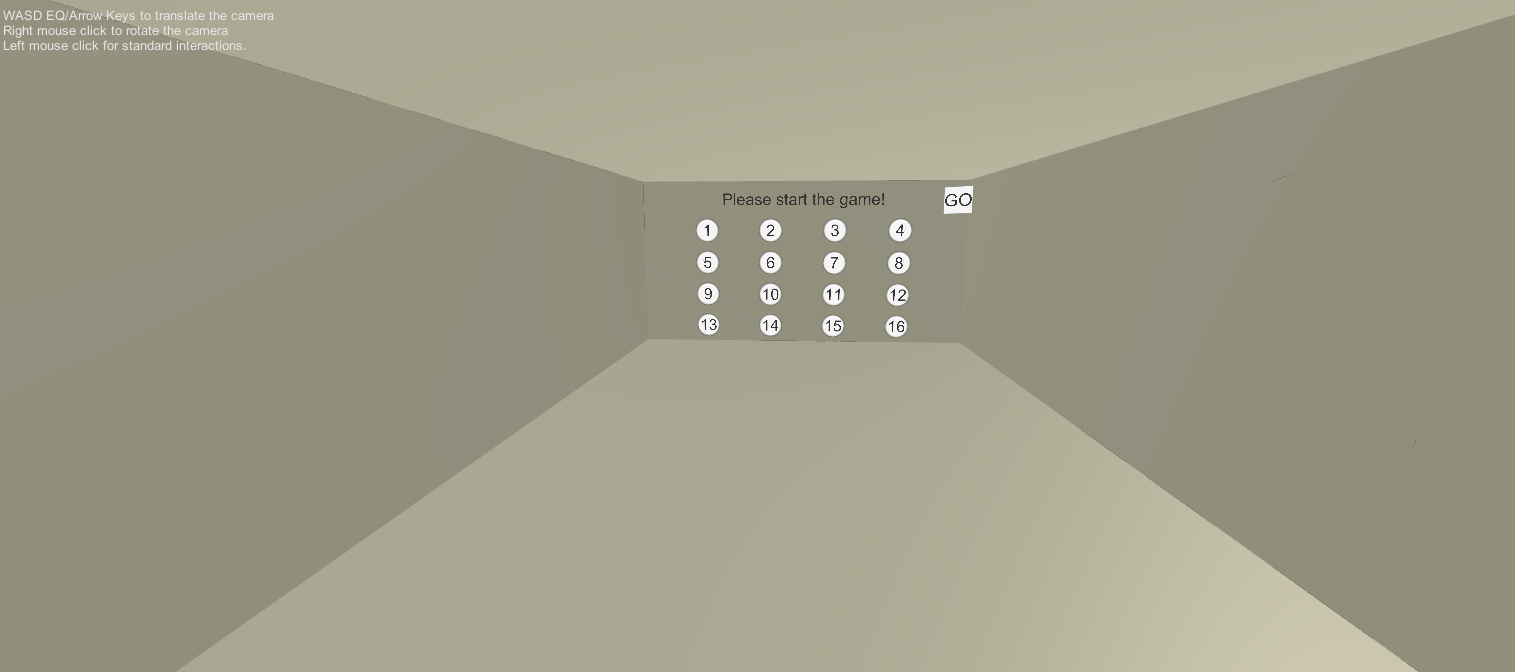
\includegraphics[width=1\linewidth]{FittsLawFurther}
	\caption[Szene FittsLawFurther]{Szene FittsLawFurther}
	\label{fig:FittsLawFurther}
\end{figure}

Bei den ersten drei Szenen ist die Spielfläche zweidimensional. Die Spielfläche befindet sich an der Wand und die Bedienelemente befinden sich auf der gleichen Ebene an der Wand. In der vierten und letzten Szene \glqq 3D-Level\grqq{} (siehe \autoref{fig:3D-Level}) wird untersucht, welche Auswirkungen eine dreidimensionale Spielfläche auf das Eye-Tracking hat. Die Bedienelemente befinden sich nicht mehr auf der gleichen Ebene, sondern schweben im Raum. Die Entfernung zwischen dem Benutzer und den Bedienelementen variiert von 4,5 bis 9,5 \ac{u}. Der interessante Aspekt an dieser Szene ist, dass gegebenenfalls ein Bedienelement zum Teil ein anderes Bedienelement verdeckt. Hierbei wird insbesondere die Zuverlässigkeit des Eye-Trackings auf die Probe gestellt. 

\begin{figure}[!htbp]
	\centering
	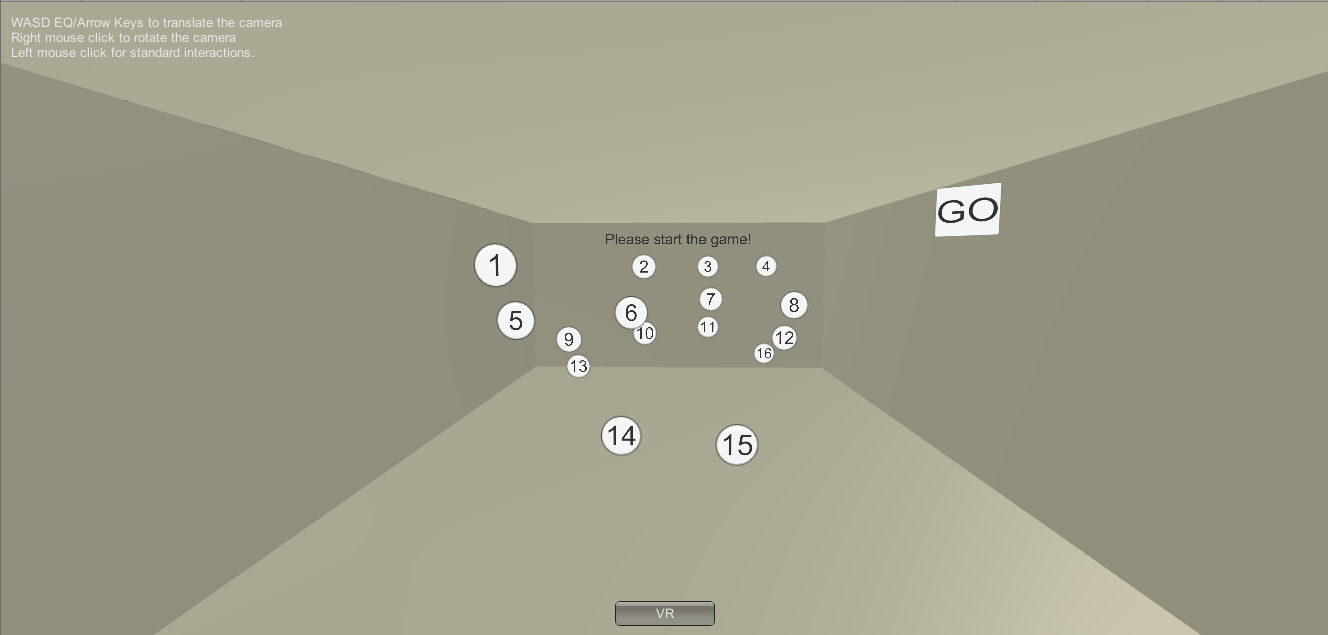
\includegraphics[width=1\linewidth]{3dlevel}
	\caption[Szene 3D-Level]{Szene 3D-Level}
	\label{fig:3D-Level}
\end{figure}

\section{Steuerung}
\label{section:controls}
Um beurteilen zu können, ob sich Eye-Tracking zur Steuerung von Bedienelementen in \ac{VR} eignet, werden verschiedene Steuerungsmöglichkeiten getestet. Die Steuerung innerhalb der \ac{VR}-Umgebung kann mit den Controllern erfolgen und mit Eye-Tracking. Die Steuerung lässt sich in Anvisieren und Interagieren unterteilen. Damit beim Anvisieren von Elementen mit dem Controller für den Benutzer klar wird, in welche Richtung der Controller zeigt, wird für das Anvisieren der Controller mit einem Laserpointer versehen. Beim Eye-Tracking wird der anvisierte Punkt durch den GazeVisualizer (vgl. \autoref{fig:GazeVisualizer}) dargestellt. Das Interagieren mit dem Controller erfolgt durch den Abzug auf der Unterseite des Controllers. Beim Eye-Tracking erfolgt dies durch Blinzeln.

Anhand dieser Kenntnisse lassen sich die Steuerungsmöglichkeiten in drei Gruppen aufteilen. Die erste Gruppe ist die Steuerung mit den \ac{VR}-Headset Controllern. Die Controllervariante ist die klassische Steuerungsmöglichkeit. In der Regel benötigt der Benutzer zum Interagieren mit der \ac{VR}-Umgebung mindestens einen Controller. Die zweite Gruppe ist die Steuerung mithilfe des Eye-Trackers. Bei Eye-Tracking wird der Blick zum Anvisieren verwendet und das Blinzeln zum Interagieren mit der \ac{VR}-Umgebung verwendet. Die letzte Möglichkeit ist der Mix aus der klassischen Steuerung sowie der Steuerung mithilfe des Eye-Trackings. Hier übernimmt jeweils eine Steuerungsmöglichkeit das Anvisieren und die andere das Interagieren. Daraus ergeben sich die folgenden vier Versuchskombinationen:

\begin{enumerate}
	\item \textbf{Laserpointer/Trigger}: Diese Versuchskombination verwendet die klassische Steuerelemente in \ac{VR}. Um einschätzen zu können, wie gut Eye-Tracking im Vergleich zu der klassischen Steuerungsvariante funktioniert, wird diese Versuchskombination benötigt. 
	\item \textbf{Eye-Tracking/Blinzeln}: Bei dieser Versuchskombination wird der Benutzer nur über Eye-Tracking mit der \ac{VR}-Umgebung interagieren. 
	\item \textbf{Laserpointer/Blinzeln}: Diese Versuchskombination hilft beim Feststellen, wie gut die Interaktion in \ac{VR} mit Blinzeln funktioniert. 
	\item \textbf{Eye-Tracking/Trigger}: Bei dieser Versuchskombination liegt der Fokus auf der Blickerfassung. Der Benutzer muss sich nur auf das Anvisieren eines Bedienelementes konzentrieren und mit dem Trigger am Controller die Auswahl betätigen.
\end{enumerate}

\section{Implementierung}
\begin{figure}[!htbp]
	\centering
	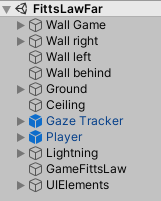
\includegraphics[width=0.4\linewidth]{scenes-structure}
	\caption[Aufbau der Szenen]{Aufbau der Szenen}
	\label{fig:scenes-structure}
\end{figure}

Die \autoref{fig:scenes-structure} zeigt exemplarisch die Objektstruktur der Szenen in Unity. Jede Szene hat elf Hauptobjekte, welchen teilweise wieder Unterobjekte zugeordnet sind. In der folgenden Aufzählung wird jedes dieser elf Hauptobjekte kurz beschrieben.

\begin{description}
	\item \textbf{Wall Game}: Das Objekt ist die Wand gegenüber des Spielers. Diese Wand ist die Spielfläche, der die Knöpfe der Wand als Unterobjekte zugeordnet sind.
	\item \textbf{Wall right / left / behind}: Diese drei Objekte sind die restlichen Wände, sodass der Spieler das Gefühl hat in einem Raum zu stehen. Auf der rechten Wand befindet sich der GO-Knopf.
	\item \textbf{Ground / Ceiling}: Die Objekte für die Decke und für den Boden sollen den Raum schließen. Auf dem Boden befindet sich als Unterobjekt das rote Quadrat, auf dem sich der Spieler vor den Versuchen zu positionieren hat.
	\item \textbf{Gaze Tracker}: Der GazeTracker enthält die relevanten Informationen für das Eye-Tracking. In diesem Objekt wird zudem die Kommunikation zum Eye-Tracker von Pupil Labs hergestellt. Zudem sind alle wichtigen Controller und der Gaze Visualizer aus dem hmd\_eyes Plugin enthalten. Das komplette GameObject ist ein Prefab, welches aus dem hmd\_eyes Plugin stammt. 
	\item \textbf{Player}: Das Spielerobjekt enthält die relevanten Informationen, welche für den Spieler wichtig sind. Dieses Objekt implementiert das Spieler-Modell von SteamVR, welches eine einfache Integration von \ac{VR} in Unity ermöglicht.
	\item \textbf{Lightning}: Das Objekt beinhaltet die Objekte für die Beleuchtung für den Raum. Für eine angenehme, gleichmäßige Beleuchtung im Raum werden zwei Point Lights verwendet. Die Lichter sind in der Mitte des Raumes jeweils einmal an der Decke und an dem Boden angebracht. 
	\item \textbf{GameFittsLaw}: Dieses Objekt beinhaltet die Spiellogik. Es ist daher nicht sichtbar in der \ac{VR}-Umgebung. 
	\item \textbf{UIElements}: Diesem Objekt sind die graphischen Elemente für die verschiedenen Einstellungen für die Versuche zugeordnet. Diese Elemente sind nur in der Unity-Übersicht sichtbar. 
\end{description}

In \autoref{fig:ClassDiagram} ist ein Überblick der für dieses Projekt generierten Klassen und der Hierarchie dargestellt. Gut zu sehen ist, dass durch Vererbung der Großteil der Klassen ein Kind der Unity eigenen Klasse {\ttfamily MonoBehaviour} ist. Nachfolgend werden die wichtigsten Objekte beziehungsweise Strukturen erläutert. 

\subsection{BaseMono}
Die für den Versuchsaufbau selbst erstellten Komponenten erben von der Basisklasse {\ttfamily BaseMono}. Diese Klasse stellt die abstrakten Methoden {\ttfamily OnCalibrationStarted} und {\ttfamily OnCalibrationRoutineDone} bereit. Die Methoden dienen als Event-Handler für die Kalibrierung. Zu Beginn der Kalibrierung wird die Methode {\ttfamily OnCalibrationStarted} aufgerufen, am Ende {\ttfamily OnCalibrationRoutineDone}. Mithilfe dieser Methoden können die Kindklassen auf den Kalibriervorgang reagieren und gegebenenfalls bestimmte Routinen ausschalten. Zusätzlich stellt {\ttfamily BaseMono} die abstrakten Methode {\ttfamily DoAwake}, {\ttfamily DoStart} und {\ttfamily DoDestroy} bereit. Diese Methoden werden von den MonoBehaviour-Funktionen {\ttfamily Awake}, {\ttfamily Start} und {\ttfamily OnDestroy} aufgerufen.

\subsection{UIElements}
Damit für jede Versuchskombination nicht eine eigene Umgebung erstellt werden muss, erhält jede Umgebung eine Einstellungsmöglichkeit für die verschiedenen Versuchskombinationen. In \autoref{fig:switch-different-options} ist die Einstellungsoberfläche für die Versuchskombinationen dargestellt. Für die Versuche können sowohl die Steuerungskombinationen als auch die Durchmesser der Knöpfe verändert werden. Zur Fixierung eines Objektes kann entweder der Laser oder das Eye-Tracking verwendet werden. Die Bestätigung kann entweder über den Trigger am Controller oder Blink Detection erfolgen. Mit dem unteren Slider lässt sich der Durchmesser der Knöpfe in drei Stufen verändern. Die Oberfläche ist nur in Unity, aber nicht in der \ac{VR}-Umgebung zu sehen.

\begin{figure}[!htbp]
	\centering
	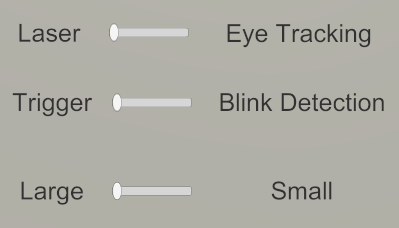
\includegraphics[width=1\linewidth]{switch-different-options}
	\caption[Einstellungsoberfläche für die Versuchsoptionen]{Einstellungsoberfläche für die Versuchsoptionen; Oben: Anvisieren; Mitte: Bestätigen; Unten: Größe der Knöpfe}
	\label{fig:switch-different-options}
\end{figure}

Sowohl für die Steuerungsmöglichkeit, als auch für die Skalierung der Knopfdurchmesser werden Enumerationen verwendet, die die verschiedenen Status darstellen. Zudem wurde zu jeder Enumeration zusätzlich eine Property-Klasse angelegt. Das Ziel der Property-Klasse ist es, die aktuell gültige Steuerungskombination, sowie die Skalierung der Knöpfe global zu sichern. Außerdem soll jede Klasse, die Kenntnisse über die Daten hat, bei Änderungen des Wertes über ein {\ttfamily PropertyChangedEvent} informiert werden. Die Klassen haben somit bei Interesse an den Werten die Möglichkeit das Event zu abonnieren. \\
Wie in \autoref{fig:ClassDiagrammProperties} zu sehen gibt es die Enumerationen {\ttfamily ControlState} und {\ttfamily Scaling}. ControlState beinhaltet die Enumerationen LaserTrigger, EyeTrigger, LaserBlinking und BlinkingEye. Scaling beinhaltet die Enumerationen Large, Medium und Small. Zu jeder Enumeration existiert zudem die passende Property-Klasse. Während {\ttfamily ControlStateProperty} nur den aktuellen Wert von ControlState speichert, wird in {\ttfamily ScalingProperty}, neben dem aktuellen Scaling Wert, zusätzlich Faktoren für die Höhe, Breite und Tiefe bei den unterschiedlichen Scalings gespeichert. Der Faktor ist bei Large eins, bei Medium dreiviertel und bei Small nur noch halb so groß.

\begin{figure}[!htbp]
	\centering
	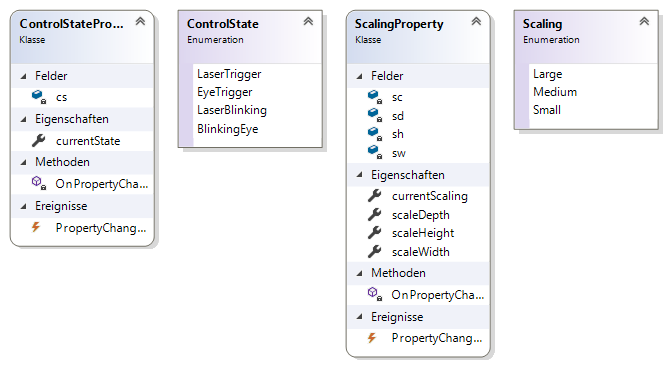
\includegraphics[width=1\linewidth]{ClassDiagramProperties}
	\caption[Klassendiagramm der ScalingProperty \& ControlStateProperty]{Klassendiagramm der ScalingProperty \& ControlStateProperty}
	\label{fig:ClassDiagrammProperties}
\end{figure}

Ein Slider feuert ein {\ttfamily OnValueChangedEvent}, sobald sich der Wert des Sliders ändert. In \autoref{lstlisting:LaserEyeTracking} ist die Methode {\ttfamily LaserEyeTrackingSliderChanged}, welche Änderungen des ersten Sliders zwischen Laser und EyeTracking abfängt. Obwohl in der Methode der neue Wert nicht mitgeliefert werden kann, kann der neue Wert gesetzt werden. Hier wird sich der Eigenschaft einer Enumeration zunutze gemacht, in der der Datentyp des Konstantenwerts der Enumerationsmember ein Integer ist \cite{BillWagner.2020}. Mithilfe von geschickter XOR Arithmetik kann der Status in ControlState gesetzt werden. Da vier Werte vorhanden sind, reichen zwei Bits aus um die Kombinationen zu erstellen. Für das Fokussieren auf ein Objekt wird die niederwertigste Bit-Stelle verwendet. Wenn das Bit 0 ist, wird der Laser zum fokussieren verwendet, bei einer 1 das Eye-Tracking. Bei der höherwertigen Bit-Stelle wird das Bestätigen der Auswahl gesetzt. Eine 0 ist das Verwenden des Abzuges, eine 1 des Blinzelns. Beim Slider für das Scaling werden dem Slider die Werte 0, 1 und 2 zugewiesen. Das aktuelle Scaling als Enumeration wird mittels Typumwandlung von Integer zur Enumeration erhalten.

\begin{lstlisting}[caption=Method LaserEyeTrackingSliderChanged,label=lstlisting:LaserEyeTracking]
public void LaserEyeTrackingSliderChanged()
{
    int state = (int)ControlStateProperty.currentState;
    state = state ^ 0b01;
    this.setControlState((ControlState)state);
}
\end{lstlisting}

\subsection{Knöpfe}
In den Szenen wird zwischen zwei Arten von Knöpfen unterschieden. Die erste Art ist der GO-Knopf, welcher beim Betätigen das Spiel startet. Die zweite Art sind die Spielknöpfe, welche mit den Zahlen für das Spiel beschriftet sind. Wie in \autoref{fig:ClassDiagramButton} zu sehen, existieren für beide Arten der Knöpfe eine Klasse, welche wiederum von der Basisklasse {\ttfamily GeneralButton} abgeleitet sind. Diese Klassen sind den jeweiligen GameObject-Buttons als Komponente zugeordnet. Die Basisklasse stellt die abstrakte Methode {\ttfamily DoAction} bereit. Diese Methode wird aufgerufen, wenn der Knopf angeklickt wurde. In der {\ttfamily DoStart} wird die {\ttfamily DoAction} als Listener für das Event {\ttfamily onClick} eines Knopfes hinzugefügt. Die beiden Kindklassen {\ttfamily ButtonNumber} und {\ttfamily ButtonGo} implementieren die {\ttfamily DoAction} Methode. Für alle Knöpfe soll nur eine Aktion passieren, wenn keine Kalibrierung des Eye-Trackers läuft. In der {\ttfamily DoAction} des GO-Knopfes wird das Spiel gestartet. Bei der Auswahl eines Spielknopfes, teilt der Knopf dem Spiel mit, dass dieser Knopf betätigt wurde. Hierfür wird dem Spiel die Nummer des betätigten Knopfs mitgeteilt. Wenn der betätigte Knopf der gesuchte Knopf ist, wird die Hintergrundfarbe des Knopfs auf grün gesetzt, ansonsten auf rot. Hiermit wird dem Benutzer visuell mitgeteilt, ob der betätigte Knopf der gesuchte wahr oder nicht. \\
Mithilfe der Klasse {\ttfamily ButtonCanvas} wird die Größe der Spielknopfs verändert. Hierfür wird das {\ttfamily PropertyChangedEvent} der {\ttfamily ScalingProperty} abonniert. Bei einer Änderung des Skalierungsfaktors wird die neue Skalierung auf die Knöpfe angewandt. In {\ttfamily ButtonCanvas} werden zudem die Knöpfe zu Beginn und am Ende des 3DLevel an der Wand positioniert. 

\begin{figure}[!htbp]
	\centering
	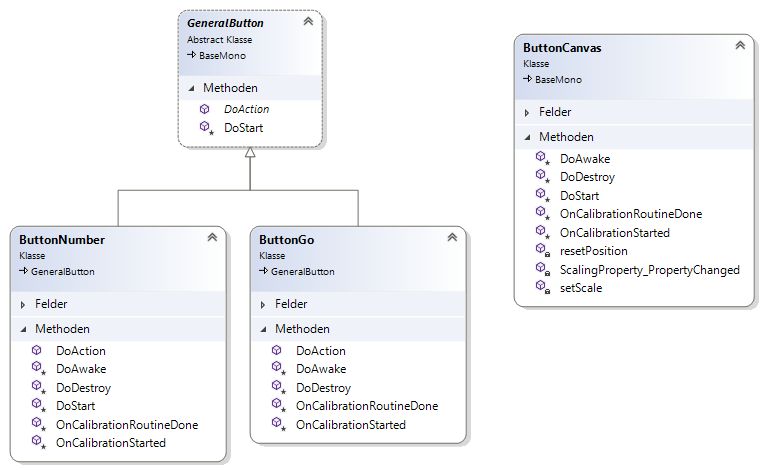
\includegraphics[width=1\linewidth]{ClassDiagramButton}
	\caption[Klassendiagramm Button]{Klassendiagramm Button}
	\label{fig:ClassDiagramButton}
\end{figure}

Zur Untersuchung von Fitts' Gesetz werden runde Knöpfe auf der Spielfläche verwendet. Knöpfe, die von Unity als {\ttfamily GameObject} zur Verfügung gestellt werden, sind nicht rund, sondern rechteckig. Daher wird für die Spielknöpfe das von Unity bereitgestellte GameObject {\ttfamily Cylinder} verwendet. Ein Problem ist, dass ein {\ttfamily Cylinder} standardmäßig keinen Collider beinhaltet. Der Entwickler \citeauthor{kode80.2016} stellt in seinem Repository UnityTools auf Github (siehe \cite{kode80.2016}) eine Lösung für dieses Problem bereit. Er stellt das Asset {\ttfamily CyllinderCollider} inklusive Editor zur Verfügung, welches einen fast runden Collider um einen Zylinder legt. Der Collider besteht aus einer Anzahl definierter rechteckiger Boxen (n), welche in dem Winkel $\alpha = \frac{180^\circ}{n}$ an dem Zylinder angebracht sind. Die Anzahl der Boxen lässt sich zwischen vier und 64 variieren.\\
In der Abbildung\autoref{fig:CylinderCollider-5} ist der Spielknopf mit dem {\ttfamily CyllinderCollider} zu sehen. Gut zu sehen sind die fünf rechteckigen Boxen, welche jeweils im Winkel von 36° angebracht sind. Der Collider ist hierbei nicht rund und ist daher minimal größer als der Zylinder. In der Abbildung\autoref{fig:CylinderCollider-63} wurde die Anzahl der Boxen auf 63 erhöht. Hier passt sich der Collider um einiges besser der Form des Zylinders an. Während der Implementierung des {\ttfamily CyllinderCollider} ist aufgefallen, dass eine höhere Anzahl an Boxen eine schlechtere Performance verursacht. Für die Versuche wird daher der {\ttfamily CyllinderCollider} mit fünf Boxen (Abbildung\autoref{fig:CylinderCollider-5}) verwendet. Nach \citeauthor{Colliders.2020} reicht dies aus, da ein unsichtbarer Collider nicht exakt die gleiche Form haben muss, sondern eine grobe Annäherung oft effizienter ist und beim Verwenden kein unterschied festgestellt werden kann \cite{Colliders.2020}. Da das System, aufgrund der Anforderungen der verwendeten Hardware, bereits stark ausgelastet ist, wird zudem eine noch höhere Auslastung des Systems vermieden.

\begin{figure}[!htbp]
	\centering
	\subfloat[5 Rechtecke\label{fig:CylinderCollider-5}]{%
		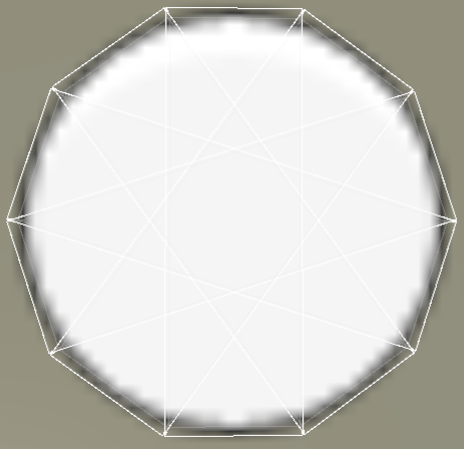
\includegraphics[height=0.45\linewidth]{CylinderCollider_5}
	}
	\qquad      
	\subfloat[63 Rechtecke\label{fig:CylinderCollider-63}]{%
		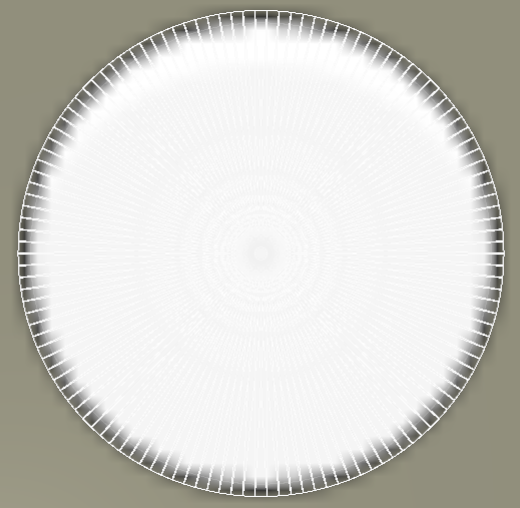
\includegraphics[height=0.45\linewidth]{CylinderCollider_63}
	}
	\caption{CyllinderCollider}
	\label{fig:CylinderCollider}
\end{figure}  

\subsection{Player}
Das GameObject {\ttfamily Player} ist ein zentrales Objekt in den Szenen. Das Objekt beschreibt den Benutzer in Unity und ist über die SteamVR-Bibliothek mit SteamVR verbunden. Das Objekt beinhaltet unter anderem die VR-Kamera und Objekte, welche die rechte beziehungsweise linke Hand, beschreiben. In den Versuchen wird ein Laserpointer und das Betätigen des Abzuges am Controller verwendet. Hierfür wird der rechten Hand die von SteamVR bereitgestellte Komponente {\ttfamily SteamVR\_LaserPointer} hinzugefügt. Mithilfe dieser Komponente wird der rechten Hand der Laserpointer hinzugefügt. Zudem ist es über diese Komponente möglich das Event {\ttfamily PointerClick} zu abonnieren, welches beim Betätigen des Abzuges ausgelöst wird. 

Dem Player ist die Klasse {\ttfamily BasePlayer} als Komponente zugeordnet, welche die komplette Steuerungslogik enthält. In Abhängigkeit der ausgewählten Steuerungsvariante werden verschiedene Events abonniert. Bei einem Wechsel der Steuerungsvariante werden die Abonnements wieder entfernt. Bei der Verwendung des Laserpointers zum Anvisieren eines Punktes wird kein Event verwendet. Stattdessen wird die Dicke des Laserstrahls angepasst, sodass der Laserstrahl nur bei den Kombinationen Laserpointer/Trigger und Laserpointer/Blinzeln sichtbar ist. Von der Laserpointer Komponente kann das Event {\ttfamily PointerClick} abonniert werden, um eine Aktion des Abzuges mitzubekommen. Das Event wird bei den Steuerungsvarianten Laserpointer/Trigger und Eye-Tracking/Trigger verwendet. Für die Verwendung des Eye-Trackings werden die Blickdaten abonniert und der {\ttfamily GazeVisualizer} sichtbar gemacht. Die Blickdaten und der {\ttfamily GazeVisualizer} werden für die Steuerungsvariante Eye-Tracking/Trigger und Eye-Tracking/Blinzeln benötigt. Als letztes abonniert die Komponente die Blinzel-Erkennung. Das Abonnieren der Blinzel-Erkennung erfolgt über den {\ttfamily RequestController} und {\ttfamily SubscriptionController}. Mithilfe des {\ttfamily RequestControllers} wird das Blinzel-Erkennungs-Plugin von Pupil Capture gestartet. Dem {\ttfamily SubscriptionsController} wird mitgeteilt, dass die Eventdaten \glqq blinks\grqq{} an die Methode {\ttfamily ReceiveBlinkData} gesendet werden sollen. Die Blinzelerkennung wird sowohl für Laserpointer/Blinzeln als auch Eye-Tracking/Blinzeln zur Bestätigung der Auswahl benötigt.

Beim Bestätigen der Auswahl über den Abzug oder das Blinzeln wird anhand des Laserpointers oder des Eye-Trackings überprüft, ob und welches Objekt anvisiert ist. Wird der Laserpointer zum Anvisieren verwendet, dann wird aus der Position des Laserpointers und der Richtung, in die der Laserpointer zeigt, das anvisierte Objekt bestimmt. Bei Eye-Tracking wird stattdessen das anvisierte Objekt mithilfe der \ac{VR}-Kamera beziehungsweise der Position des \ac{HMD} in Kombination mit der vom Eye-Tracker berechneten Blickrichtung verwendet. Um die \ac{VR}-Weltraumkoordinaten für die Blickdaten zu erhalten, muss die Blickrichtung in den Weltraum transformiert werden. In \autoref{lstlisting:CheckCollision} ist ein Ausschnitt der Methode {\ttfamily checkCollision} zu sehen, in der anhand der Position und der Richtung das anvisierte Objekt herausgefunden wird. Unity stellt die Funktion {\ttfamily Raycast} bereit, welche das erste getroffene Objekt in der Variablen {\ttfamily hit} speichert. Der Rückgabewert der Funktion ist vom Datentyp {\ttfamily bool}. Bei einem erfolgreichen Treffer gibt die Funktion {\ttfamily true}, ansonsten {\ttfamily false} zurück. Anhand des {\ttfamily GameObjects} kann ein Klick eines Knopfs durchgeführt werden.

\begin{lstlisting}[caption=Ausschnitt aus Methode checkCollision,label=lstlisting:CheckCollision]
private void checkCollision(Vector3 origin, Vector3 direction)
{
	if (Physics.Raycast(origin, direction, out RaycastHit hit))
	{
		GameObject currObject = hit.collider.gameObject;
		
		// do triggering
		// ...
	}
}
\end{lstlisting}

Das Verwenden von Blinzeln als Bestätigung ist eine Herausforderung. In \autoref{lstlisting:ReceiveBlinkData} ist die Methode {\ttfamily ReceiveBlinkData} zu sehen, welche aufgerufen wird, sobald ein Blinzeln erfasst wurde. Da beim Blinzeln sowohl das Auf- und Zugehen der Augen als Blinzeln erkannt wird, werden zwei Events an die Methode {\ttfamily ReceiveBlinkData} pro Blinzeln geschickt. Damit daher nur ein Event eines Blinzelns verarbeitet wird, wird eine Coroutine verwendet. Hierfür wird die Mehode {\ttfamily Blink} in einer Coroutine ausgeführt. In \autoref{lstlisting:Blink} ist die Methode zu sehen, welche das Bestätigen durch Blinzeln durchführt. Nach dem der Kollisionscheck durchgeführt wurde, muss die Coroutine eine definierte Dauer von 250ms warten, bis sie sich beendet und den nachfolgenden Code ausführt. Die Flags {\ttfamily onBlinking} und {\ttfamily blinking} unterbinden, dass aufgrund des Blinzelns mehrere Coroutinen ausgeführt werden und die Blink-Methode mehrfach ausgeführt wird.

\begin{lstlisting}[caption=Methode ReceiveBlinkData,label=lstlisting:ReceiveBlinkData]
private void ReceiveBlinkData(string topic, Dictionary<string, object> dictionary, byte[] thirdFrame = null)
{
	if (!this.onBlinking)
	{
		this.StartCoroutine(this.Blink(this.blinkDuration));
	}
}
\end{lstlisting}

\begin{lstlisting}[caption=Ausschnitt aus Methode Blink,label=lstlisting:Blink]
public IEnumerator Blink(float duration)
{
	if (!this.blinking)
	{
		this.onBlinking = true;
		this.blinking = true;
		
		// do check collision
		
		yield return new WaitForSecondsRealtime(duration);
		this.onBlinking = false;
		this.blinking = false;
	}
	
	yield break;
}
\end{lstlisting}

\subsection{Measurement}
\label{section:measurement}
Um einen Vergleich zwischen den Steuerungsmöglichkeiten ziehen zu können, werden die Versuche aufgezeichnet. In \autoref{fig:ClassDiagramMeasurement} ist der Ausschnitt der Klassen für die Measurements zu sehen. Zu jeder Messung wird das aktuelle Level, die verwendete Steuerungskombination sowie die Skalierung der Knöpfe eines Versuchs gespeichert. Am Anfang sowie am Ende der Messung wird jeweils der aktuelle Zeitpunkt gespeichert. Hierdurch ist es möglich, die Dauer des Versuchs zu berechnen. Die Zeit wird in der Messung als Zeitstempel in Millisekunden gesichert. In dem Feld {\ttfamily action} werden die durch den Benutzer getätigten Bestätigungen durch den Abzug beziehungsweise mithilfe von Blinzeln erfasst. Hierbei wird der Zeitstempel, die Nummer des Knopfs, sowie ob es der gesuchte Knopf war, gespeichert. Das Betätigen der Spielwand wird wie das Betätigen eines Knopfs behandelt und aufgezeichnet. Als Nummer erhält die Wand eine -1. Hierdurch wird in den Messungen hervorgehoben, dass das getroffene Objekt die Spielwand war. Die Daten werden als String mit Komma getrennt in einer Liste gespeichert. Für Fitts' Gesetz ist bei der Verwendung von Eye-Tracking der Verlauf des Blickes interessant. Aus diesem Grund wird der Blickverlauf mit gemessen. Die Blickdaten werden ebenfalls in einer Liste bestehend aus Strings gespeichert. Da die Blickdaten als 3D-Vektor vorliegen, werden die Koordinaten des durch den Blick fixierten Punktes mit Komma getrennt aufgezeichnet. Alle 100 ms werden die Blickdaten erfasst und gesichert. Als Datengrundlage für die Blickverfolgung dient der Gaze Visualizer vom Gaze Tracker. Für das 3D-Level werden zusätzlich die Positionen der Knöpfe aufgezeichnet. Dies wird benötigt, da sich die Position der Knöpfe im Raum von Versuch zu Versuch unterscheiden. Für die Zuordnung, welcher Knopf auf welcher Position steht, werden zusätzlich die Nummern der Knöpfe mit gespeichert.

\begin{figure}[!htbp]
	\centering
	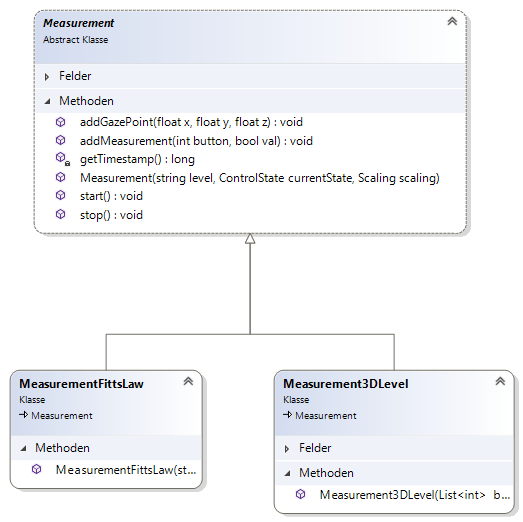
\includegraphics[width=0.65\linewidth]{ClassDiagramMeasurement}
	\caption[Klassendiagramm Measurements]{Klassendiagramm Measurements}
	\label{fig:ClassDiagramMeasurement}
\end{figure}

Jede Messung wird am Ende eines Versuchs in einer JSON-Datei abgespeichert. Die Basisklasse Measurement ist mit dem Attribut Serializable gekennzeichnet. Dies ermöglicht das Serialisieren des kompletten Measurement-Objekts. Damit alle Messdaten mit dem Objekt serialisiert werden, müssen die Felder als öffentlich gekennzeichnet sein. Das Serialisieren in ein JSON-String wird mithilfe der von Unity bereitgestellten Klasse {\ttfamily JsonUtility} durchgeführt. Für eine Gliederung der Messungen werden die Messungen in unterschiedlichen Ordnern nach Level und verwendeter Skalierung getrennt gespeichert. Der Dateiname ist zudem der Zeitstempel zum Zeitpunkt des Speichervorganges der Messung.

\subsection{Game}
\label{section:game}
Das GameObject {\ttfamily Game} beinhaltet die gesamte Spiellogik der Versuchsumgebungen. Das GameObject ist in der \ac{VR}-Umgebung für den Benutzer nicht sichtbar. Dem GameObject ist die Klasse {\ttfamily BaseGame} als Komponente zugeordnet, worin die Spiellogik implementiert ist. Sie stellt die öffentliche Methode {\ttfamily startGame} bereit, welche bei dem Betätigen des GO-Knopfs aufgerufen wird. Beim Starten eines Spiels wird ein neues Measurement angelegt, die zu suchenden fünf Zahlen ausgewählt, sowie die Farbe der Spielknöpfe zurück auf weiß gesetzt. Zudem erhält der Nutzer auf der Anzeige die erste Aufforderung, welche Zahl ausgewählt werden soll. Als Letztes wird beim Starten eines Spiels die zeitliche Messung gestartet. Über die öffentliche Methode {\ttfamily objectClicked} teilen die Spielknöpfe, sowie die Spielwand, dem Spiel mit, dass sie betätigt wurden. Die Methode {\ttfamily objectClicked} ist in \autoref{lstlisting:objectClicked} dargestellt. Damit das Spiel bewerten kann, ob der richtige Knopf betätigt wurde, wird die Nummer mit übergeben. In der Liste mit den zu suchenden Zahlen wird überprüft, ob der betätigte Knopf der Gesuchte war oder nicht. Wenn ja, wird die Knopfnummer als erfolgreich in den Messungen mit aufgenommen. Zudem wird die Zahl aus den zu suchenden Zahlen entfernt und der Anzeigetext aktualisiert. Wenn der betätigte Knopf nicht der gesuchte Knopf ist, dann wird dies entsprechend in den Messungen dokumentiert. Da es vorkommen kann, dass der Benutzer vor dem Starten des Spiels einen Spielknopf betätigt, muss überprüft werden, ob ein Measurement-Objekt bereits erstellt wurde. Da die Liste mit den gesuchten Zahlen vor dem Spielstart leer ist, reicht die Überprüfung im Fehlerfall. Am Ende der Methode teilt das Spiel dem betätigten Objekt mit, ob es das gesuchte Objekt war oder nicht. Anhand des Rückgabewertes kann der Knopf seine Farbe ändern. Wenn die letzte Zahl erfolgreich ausgewählt wurde wird das Spiel beendet. Die Messung wird dabei gestoppt und gespeichert.\\


\begin{lstlisting}[caption=Methode objectClicked,label=lstlisting:objectClicked,float=!htbp]
public bool objectClicked(int number)
{
	bool retVal;
	
	if (this.searchValues.IndexOf(number) == 0)
	{
		this.measurement.addMeasurement(number, true);
		this.searchValues.Remove(number);
		this.setInstruction();
		retVal = true;
	}
	else
	{
		if(this.measurement != null)
		{
			this.measurement.addMeasurement(number, false);
		}
	
		retVal = false;
	}
	
	return retVal;
}
\end{lstlisting}

Die Komponente BaseGame abonniert die Blickdaten vom {\ttfamily GazeController}, um diese in die Messungen mit aufzunehmen. Zudem wird das {\ttfamily PropertyChangedEvent} von ControlState abonniert, um bei Änderungen das laufende Spiel abzubrechen. Zudem wird dem Benutzer mitgeteilt, dass das Spiel abgebrochen wurde. Zusätzlich beinhaltet {\ttfamily BaseGame} die abstrakten Methoden {\ttfamily createMeasurement} und {\ttfamily getSearchValues}, welche von den Kindkomponenten {\ttfamily GameFittsLaw} und {\ttfamily Game3DLevel} implementiert wird. Mit der Methode {\ttfamily createMeasurement} werden die Versuchsumgebung-spezifischen Measurement-Objekte erzeugt. In der Methode {\ttfamily getSearchValues} werden die zu suchenden Zahlen ausgewählt. Während für das 3DLevel die zu suchenden Zahlen zufällig ausgewählt werden, sind diese für die FittsLaw-Umgebungen pseudozufällig. Hier wird zufällig ein vordefiniertes Muster ausgewählt. Die Muster haben alle das gleiche Grundmuster, nur gespiegelt oder versetzt. In \autoref{table:testcases} sind die Muster dargestellt. Die Reihenfolge der Zahlen entspricht der Suchreihenfolge. Das zweite Muster ist vertikal gespiegelt zum ersten Muster. 

\begin{table}[!htbp]
	\centering
	\caption{vordefinierte Muster}
	\label{table:testcases}
	\begin{tabular}{|c ||c c c c c|} 
		\hline
		1. & 2 & 1 & 16 & 12 & 10 \\ 
		\hline
		2. & 3 & 4 & 13 & 9 & 11 \\
		\hline
		3. & 7 & 15 & 13 & 4 & 3 \\
		\hline
		4. & 8 & 16 & 1 & 4 & 13 \\
		\hline
		5. & 5 & 6 & 14 & 8 & 13 \\
		\hline
	\end{tabular}
\end{table}

Für das 3DLevel müssen die Knöpfe zufällig in der Tiefe variiert werden. Hierfür werden beim Initialisieren eines Spiels alle Knöpfe positioniert. Knopf 1 und 16 haben eine feste Position. Knopf 1 befindet sich 5\ac{u} vor der Spielwand, Knopf 16 direkt auf der Spielwand. Die restlichen Knöpfe werden zufällig zwischen 0 und 5 \ac{u} positioniert.